\documentclass[twocolumn]{article}
\usepackage{url}
\usepackage{titling}
\usepackage{graphicx}
\usepackage[utf8]{inputenc}
\usepackage{array,etoolbox}
\usepackage[justification=centering]{caption}
\usepackage[acronym,nomain,nonumberlist,nogroupskip,nopostdot]{glossaries}

% loads the list of abbreviations
\makeglossaries
\loadglsentries{acronym}

% centers the title page
\renewcommand\maketitlehookd{\vfill\null}
\renewcommand\maketitlehooka{\null\mbox{}\vfill}

% keywords command
\providecommand{\keywords}[1]
{
  \small
  \noindent \textbf{\textit{Keywords ---}} #1
}

% counter for table
\preto\tabular{\setcounter{magicrownumbers}{0}}
\newcounter{magicrownumbers}
\newcommand\rownumber{\stepcounter{magicrownumbers}\arabic{magicrownumbers}}


\title{\gls{asl}\\
	Fingerspelling Detection}
\author{Shoaib Mohammed}
\date{01 June 2021}


\begin{document}

\begin{titlingpage}
\maketitle
\end{titlingpage}

\begin{abstract}
Approximately 70 million people around the world are deaf-mute. While 
translation services have become easily accessible for about 100 
languages, sign language is still an area that has not been explored. 
Our goal is to detect \& translate the letters of \gls{asl} in real-time.
\end{abstract}

\keywords{\gls{asl}, fingerspelling, \gls{cnn}, transfer learning, 
computer vision}


\section{Introduction}

\subsection{Background}
According to the \gls{csd} \cite{csd}, there are 360 million deaf people 
worldwide. Another report by the \gls{who} [2] bumps up the number to 466 
million people suffering from disabling hearing loss. Future projections 
estimate 630 million people by 2030 and over 900 million people by 2050. 
But even in this age of technology and communication, we are yet to see a 
universal translation system that helps bridge the gap between people that 
can and cannot speak. The goal of this project is to detect and accurately 
translate the letters in \gls{asl}.

\subsection{Scope \& Limitations}
% (TODO: do we want to add acronyms for US & UK?)
The bottom line is that there is no universal sign language. For instance, the 
\gls{bsl} differs by a great margin from the \gls{asl}. Generally speaking, a 
person in the US can understand spoken English in the UK but this is not the 
case with sign language.

% (TODO: add a reference to the statistic for more than 200 sign languages)
It is interesting to note that there are more than 200 sign languages that are 
used across the world. However, if an accurate model was developed to 
recognize a sign language, in our case, \gls{asl}, the same methodology could be 
applied to recognize other sign languages. Perhaps the major limitation is 
classifying each sign from the sheer corpus of signs in \gls{asl}.
% (TODO: add a reference showing why it’s a sheer corpus)
However, since our focus is classifying the alphabets alone, our range is 
limited to 24 alphabets since we exclude the alphabets J \& Z since these 
require motion.

\section{Literature Survey}

\subsection{Population Statistics}
A combined study in \cite{mitchell2006many} estimates there were more than 
250,000 deaf people and as many as 500,000 people who used \gls{asl} in 1972. 
Over the years, this number has been on the rise.

\begin{figure}[h]
\centering
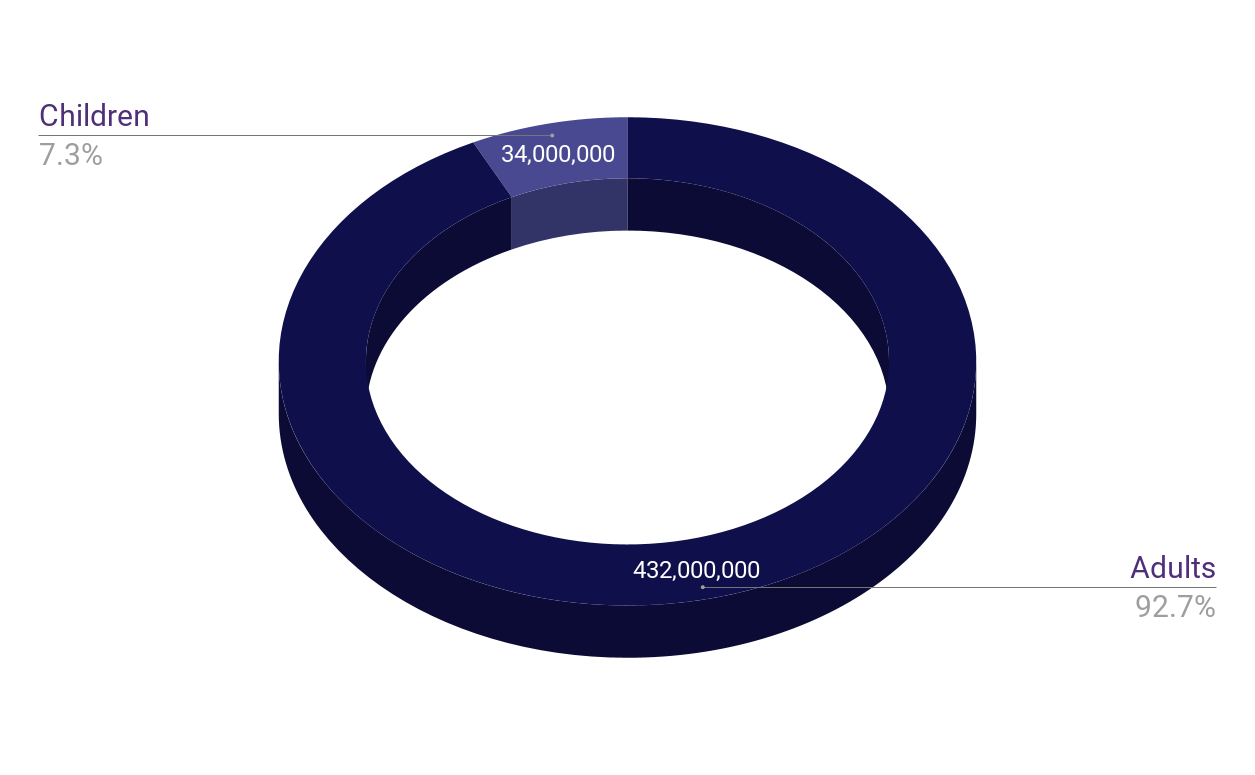
\includegraphics[width=8cm]{./figures/Distribution of the population}
\caption{Distribution of the population}
\end{figure}

\gls{sipp} collects data for the US population. From the research of 
Ross E. Mitchell \cite{mitchell2006many} in the year 2006, fewer than 1 in 20 
Americans or 10,000,000 people suffered from hard of hearing and close to 
1,000,000 were classified as functionally deaf.

\bibliographystyle{ieeetr}
\bibliography{biblio}

\listoffigures

\glsaddall
\setlength{\glsdescwidth}{0.8\textwidth}
\printglossary[type=\acronymtype,title=List Of Abbreviations]

% (TODO: cite image to the website https://www.javatpoint.com/serialization-in-java)
\begin{figure}[h]
\centering
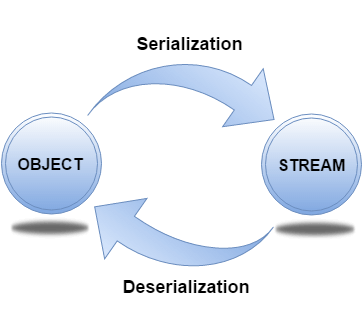
\includegraphics[width=8cm]{./figures/serialization and deserialization}
\caption{Process of serialization \& deserialization}
\end{figure}

\begin{figure}[h]
\centering
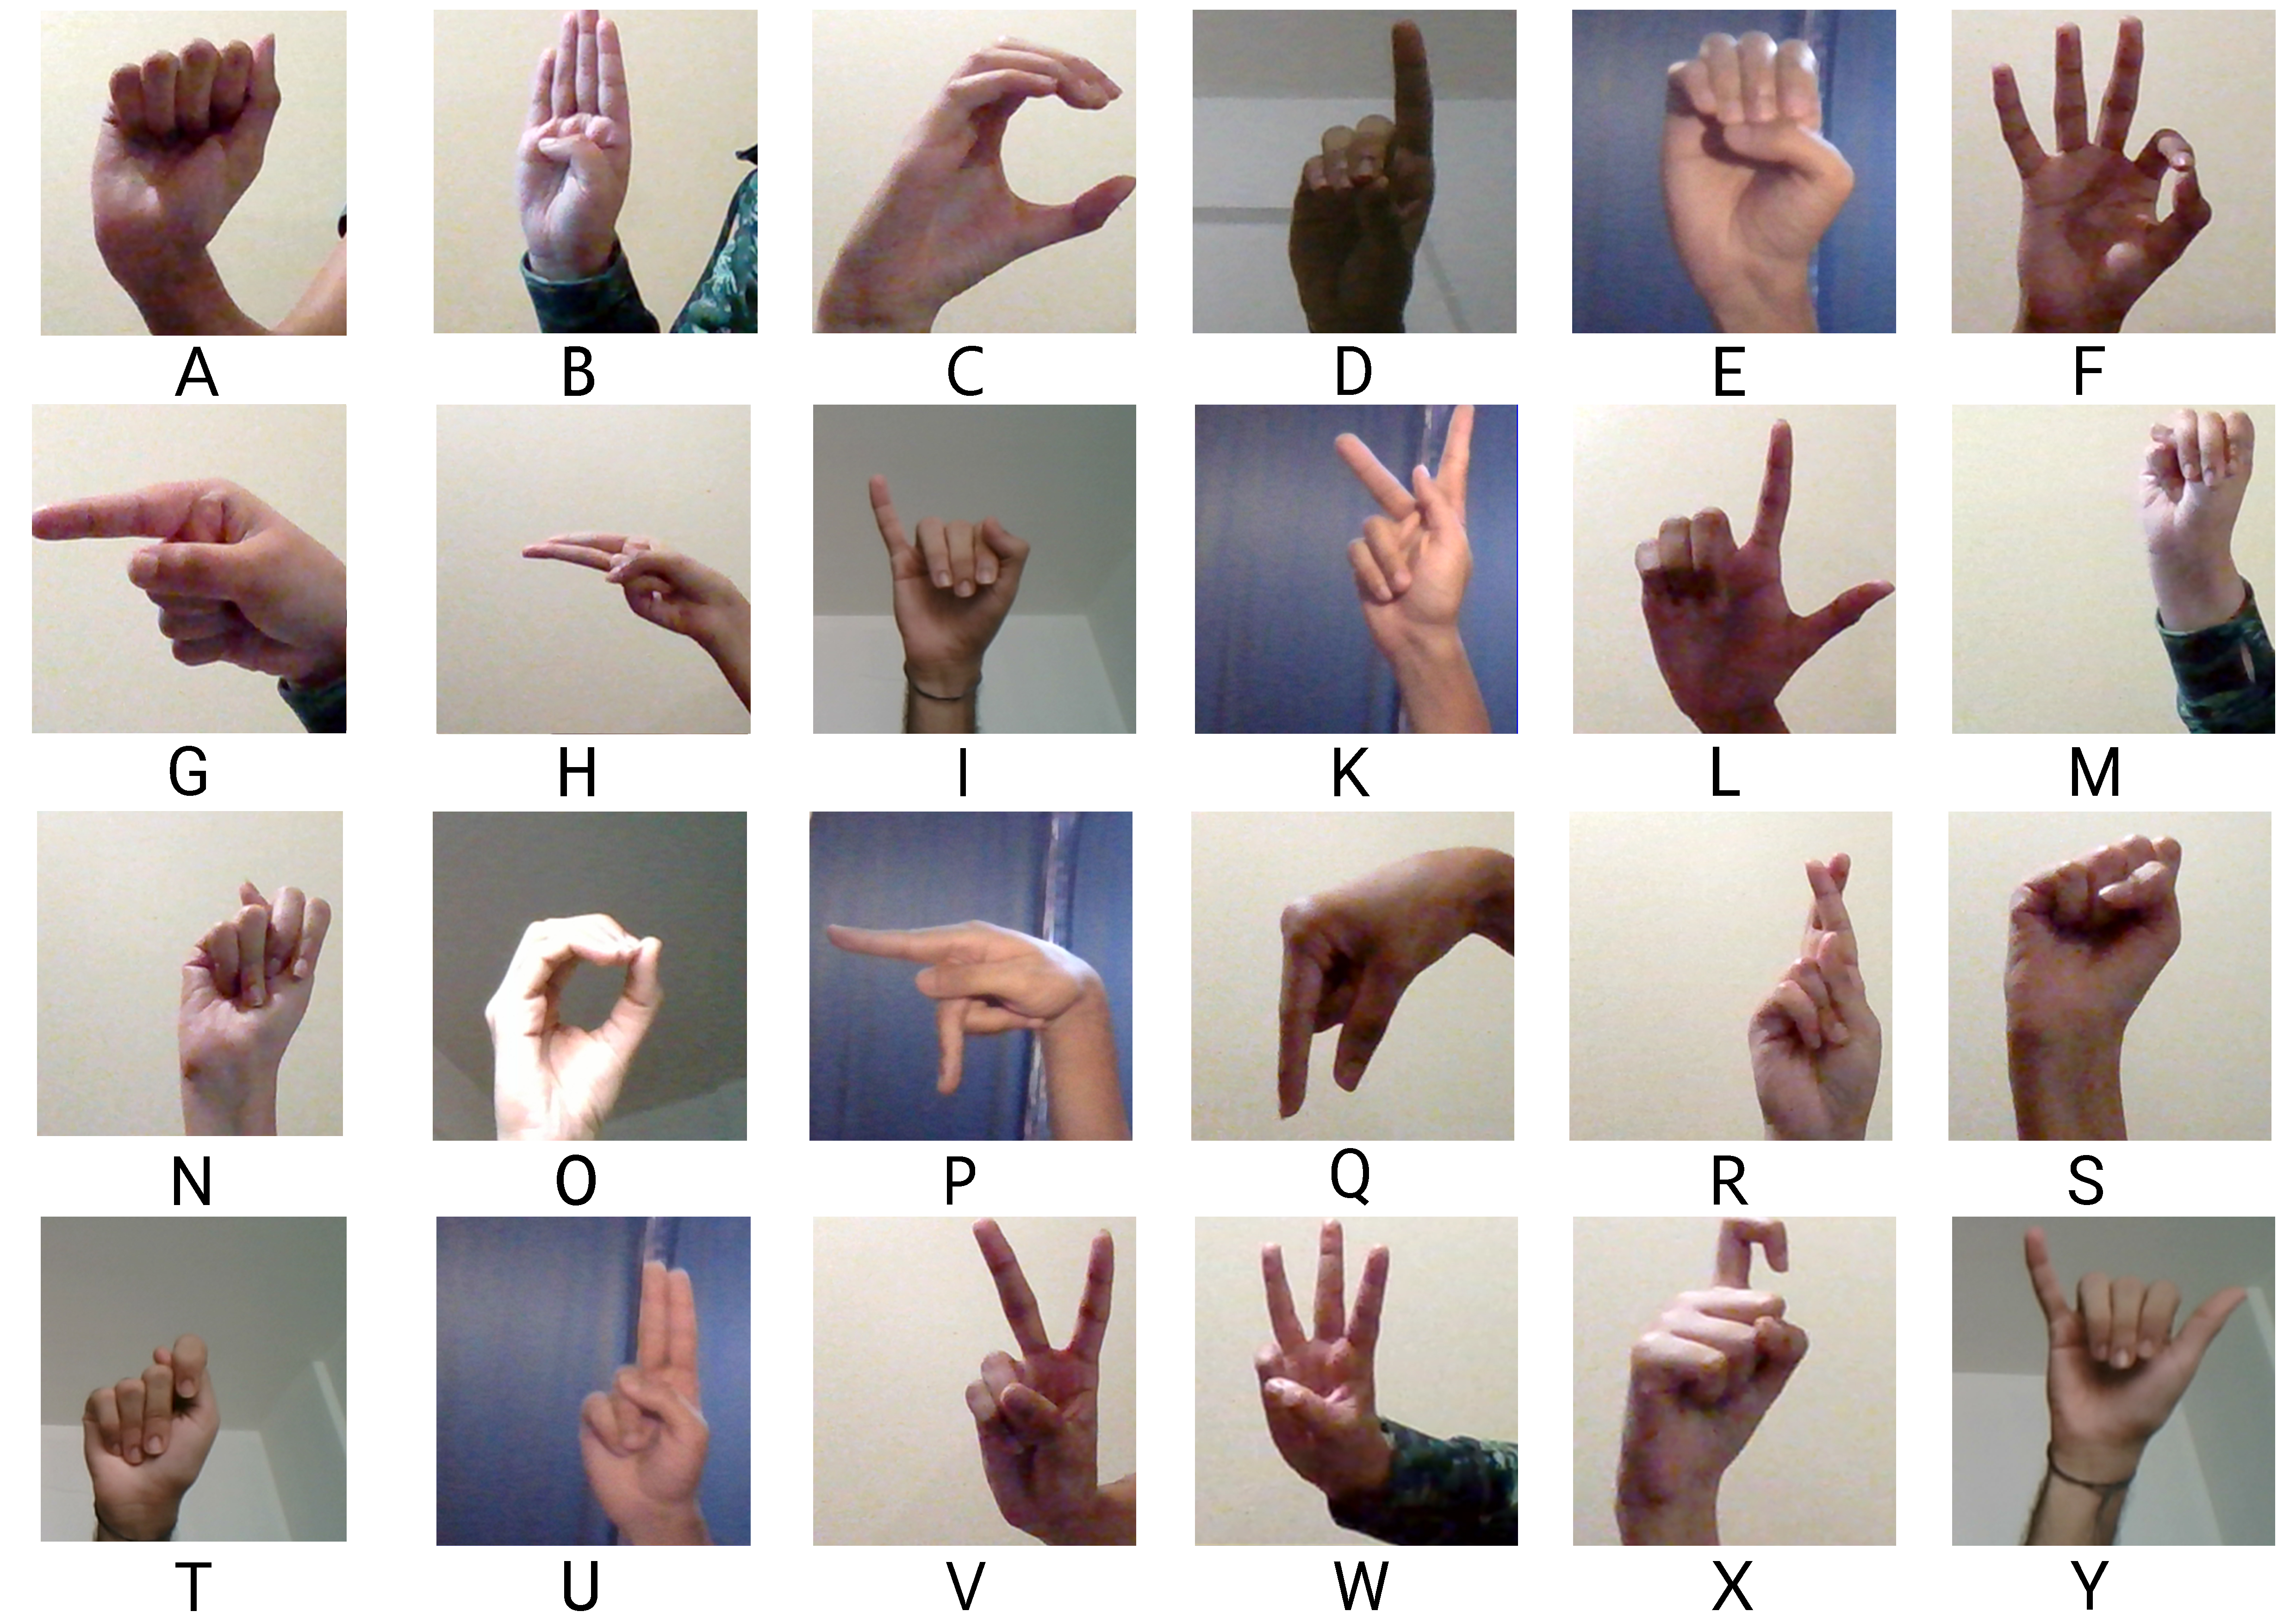
\includegraphics[width=8cm]{./figures/alphabets}
\caption{ASL alphabets from our dataset}
\end{figure}

% (TODO: cite image to the website https://medium.datadriveninvestor.com/introducing-transfer-learning-as-your-next-engine-to-drive-future-innovations-5e81a15bb567)
\begin{figure}[h]
\centering
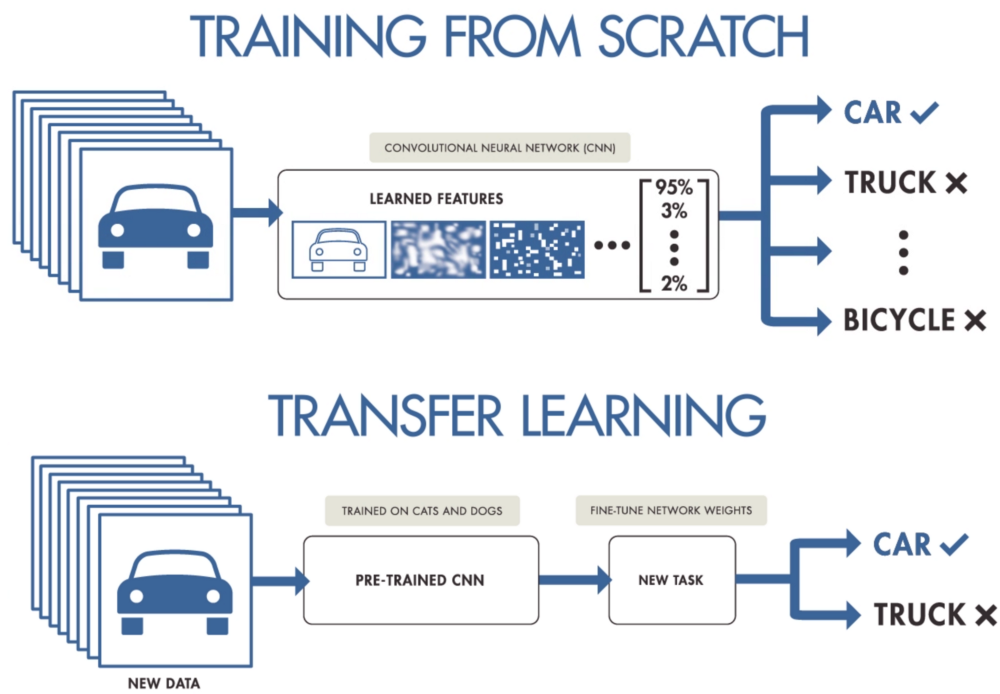
\includegraphics[width=8cm]{./figures/training from scratch vs. transfer learning}
\caption{Training from scratch vs. transfer learning}
\end{figure}

% (TODO: cite image to the website https://medium.com/@lorenzofamiglini/transfer-learning-with-deep-learning-machine-learning-techniques-b4052befe7e2)
\begin{figure}[h]
\centering
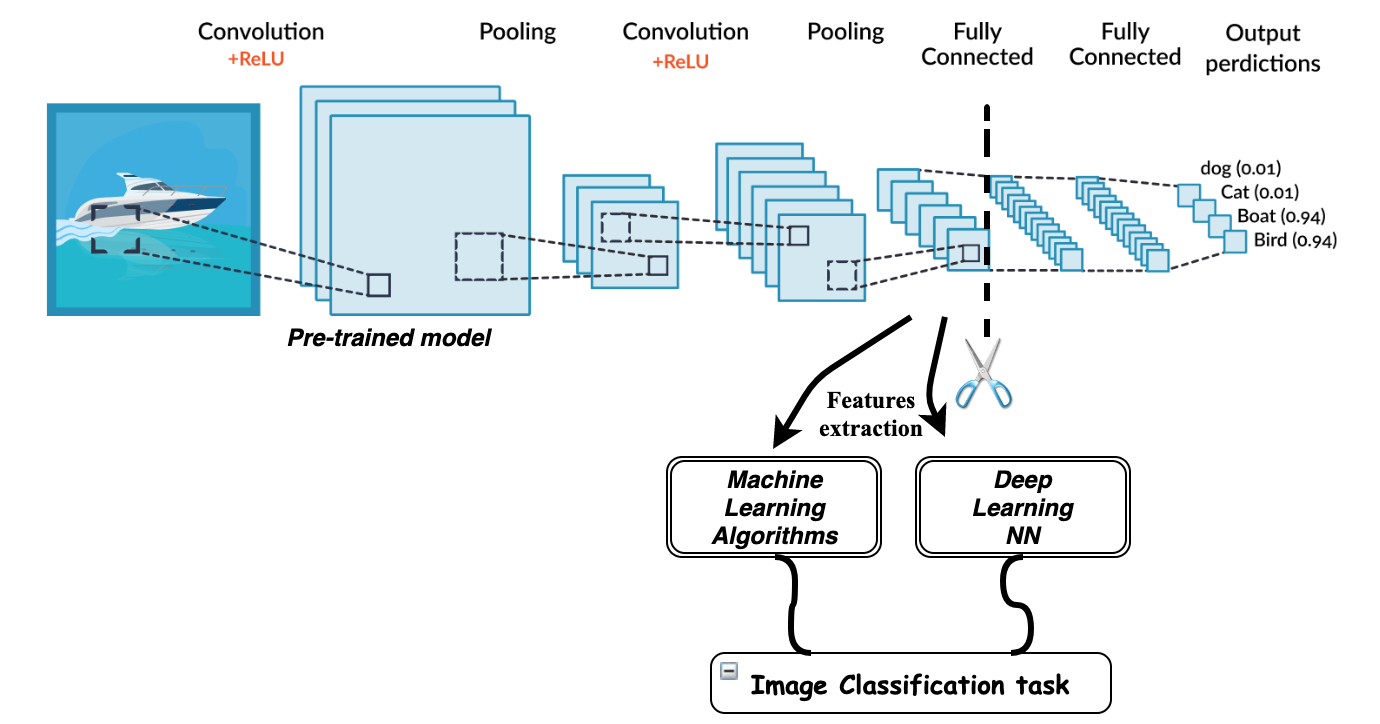
\includegraphics[width=8cm]{./figures/transfer learning process}
\caption{Transfer learning process}
\end{figure}

% (TODO: cite image to the website https://www.quora.com/What-is-the-benefit-of-using-average-pooling-rather-than-max-pooling)
\begin{figure}[h]
\centering
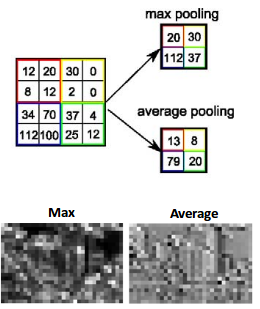
\includegraphics[width=8cm]{./figures/max pooling vs. average pooling}
\caption{Max pooling vs. Average pooling}
\end{figure}

% (TODO: cite image to the website https://medium.com/analytics-vidhya/understanding-a-single-neurons-role-in-neural-network-77bb3251e9db)
\begin{figure}[h]
\centering
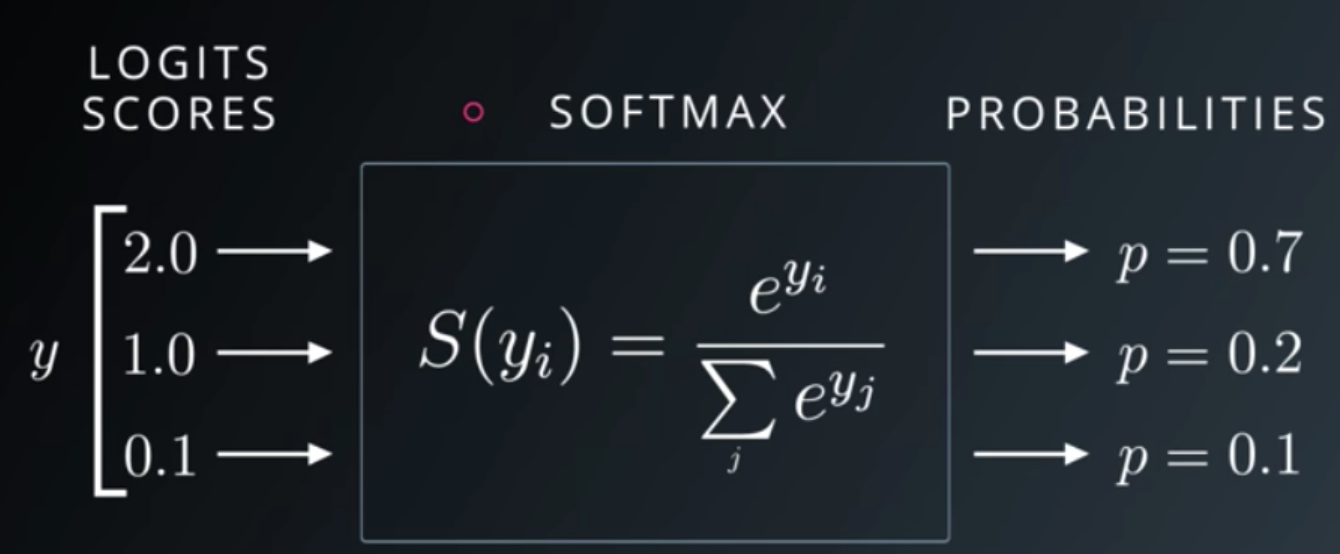
\includegraphics[width=8cm]{./figures/softmax function}
\caption{Softmax function pushing high scores close to 1 and low scores close to 0}
\end{figure}

\begin{figure}[h]
\centering
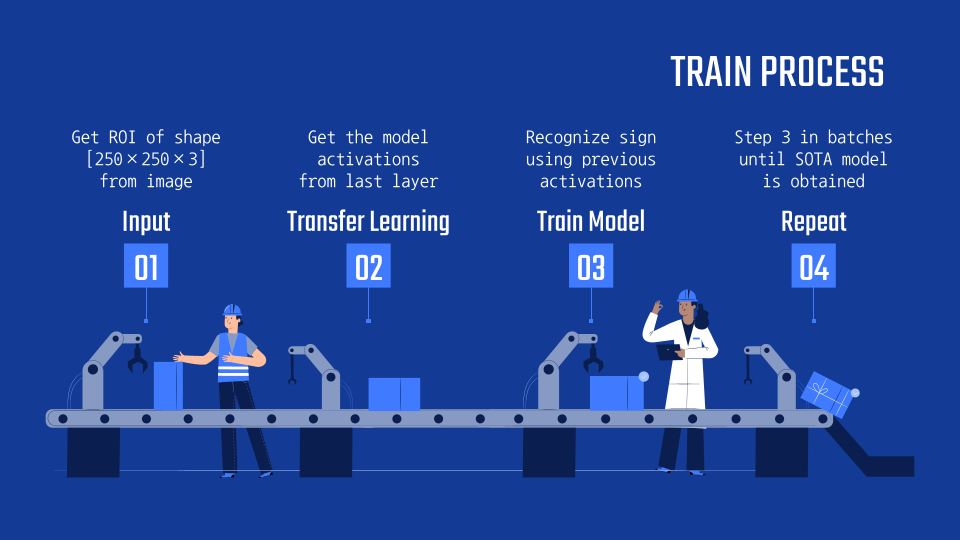
\includegraphics[width=8cm]{./figures/train process}
\caption{Process of training the model}
\end{figure}

\begin{figure}[h]
\centering
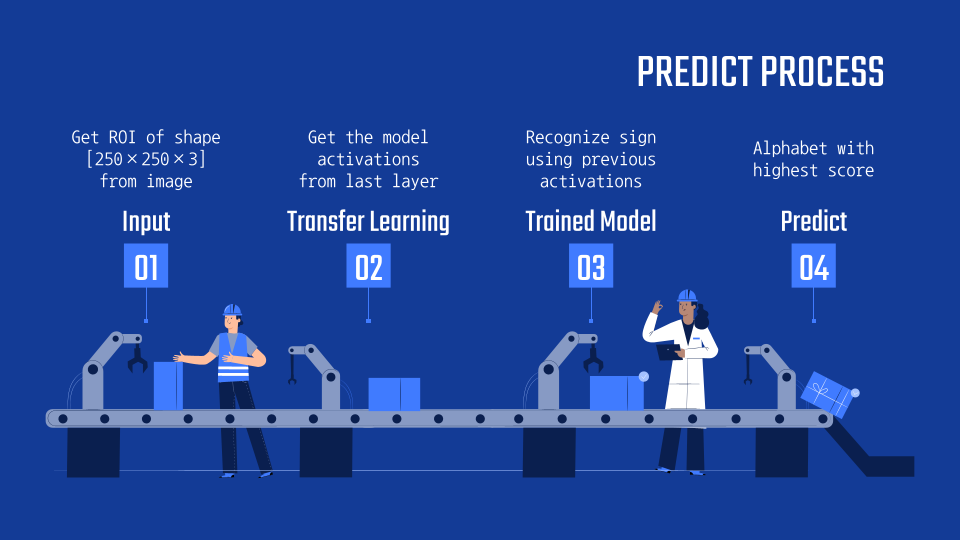
\includegraphics[width=8cm]{./figures/predict process}
\caption{Process of testing the model}
\end{figure}

\begin{table}[h]
\begin{tabular}{ |l|c|c|c| }
  \hline
  Model & Size & Accuracy & Parameters \\ \hline
  MobileNetV2 & 14 MB & 0.713 & 3,538,984 \\ \hline
  InceptionV3 & 92 MB & 0.779 & 23,851,784 \\ \hline
  Xception & 88 MB & 0.790 & 22,910,480 \\ \hline
  InceptionResNetV2 & 215 MB & 0.803 & 55,873,736 \\
  \hline
\end{tabular}
\caption{Transfer learning model statistics}
\end{table}

\begin{table}[h]
\begin{tabular}{ |l|c|c|c| }
  \hline
  Model & Size & Accuracy & Parameters \\ \hline
  MobileNetV2 & 91 MB & 0.918 & 7,934,872 \\ \hline
  InceptionV3 & 99 MB & 0.924 & 8,598,424 \\ \hline
  Xception & 100 MB & 0.908 & 8,721,304 \\ \hline
  InceptionResNetV2 & 93 MB & 0.848 & 8,074,136 \\
  \hline
\end{tabular}
\caption{Trained model statistics using varying transfer learning models}
\end{table}

\begin{table}[h]
\begin{tabular}{ | @{\makebox[2em][r]{\rownumber\space}} |l|c| }
  \hline
  \multicolumn{1}{ | @{\makebox[2em][r]{\textbf{ ID }}} |l| }{\textbf{Layer (Type)}} 
  & \multicolumn{1}{ |c| }{\textbf{Number of Parameters}} \\ \hline
  \texttt{dense\_1 (Dense)} & \emph{dependent} \\ \hline
  \texttt{dense\_2 (Dense)} & 524,800 \\ \hline
  \texttt{dense\_3 (Dense)} & 131,328 \\ \hline
  \texttt{dense\_4 (Dense)} & 32,896 \\ \hline
  \texttt{up\_sampling2d\_1 (UpSampling2D)} & 0 \\ \hline
  \texttt{conv2d\_5 (Conv2D)} & 131,136 \\ \hline
  \texttt{depthwise\_conv2d\_1 (DepthwiseConv2D)} & 1,088 \\ \hline
  \texttt{up\_sampling2d\_2 (UpSampling2D)} & 0 \\ \hline
  \texttt{depthwise\_conv2d\_2 (DepthwiseConv2D)} & 1,088 \\ \hline
  \texttt{conv2d\_6 (Conv2D)} & 65,600 \\ \hline
  \texttt{dense\_5 (Dense)} & 8,320 \\ \hline
  \texttt{dense\_6 (Dense)} & 33,024 \\ \hline
  \texttt{dense\_7 (Dense)} & 131,584 \\ \hline
  \texttt{dense\_8 (Dense)} & 525,312 \\ \hline
  \texttt{dense\_9 (Dense)} & 2,099,200 \\ \hline
  \texttt{dense\_10 (Dense)} & 2,098,176 \\ \hline
  \texttt{dense\_11 (Dense)} & 524,800 \\ \hline
  \texttt{dense\_12 (Dense)} & 131,328 \\ \hline
  \texttt{dense\_13 (Dense)} & 32,896 \\ \hline
  \texttt{max\_pooling2d\_1 (MaxPooling2D)} & 0 \\ \hline
  \texttt{flatten\_1 (Flatten)} & 0 \\ \hline
  \texttt{dense\_14 (Dense)} & \emph{dependent} \\
  \hline
\end{tabular}
\caption{Model architecture and number of parameters in each layer}
\end{table}

\end{document}
